\documentclass[12pt]{article}

\usepackage{hyperref}
\usepackage[utf8]{inputenc}
\usepackage{graphicx}
\graphicspath{ {images/} }

\title{Artifical Intelligence}
\author{
        Henry Huck \\
        Master Specialisé - HEC \\
        \and
        Romain Lapeyre\\
        Grande Ecole - HEC\\
}
\date{\today}

%%%%%%%%%%%%%%%%%%%%%%%%%%%%%%%%%%%%%%%%%%%%%%%%%%%%%%%%%%%%%%%%%%%%%%%%%%%%%%%%
%%%%%%%%%%%%%%%%%%%%%%%%%%%%%%%%%%%% Title Page %%%%%%%%%%%%%%%%%%%%%%%%%%%%%%%%
%%%%%%%%%%%%%%%%%%%%%%%%%%%%%%%%%%%%%%%%%%%%%%%%%%%%%%%%%%%%%%%%%%%%%%%%%%%%%%%%

\begin{document}

\maketitle
\thispagestyle{empty}
\pagenumbering{gobble}

\pagebreak

%%%%%%%%%%%%%%%%%%%%%%%%%%%%%%%%%%%%%%%%%%%%%%%%%%%%%%%%%%%%%%%%%%%%%%%%%%%%%%%%
%%%%%%%%%%%%%%%%%%%%%%%%%%%%%%%%%%%% Quote Page %%%%%%%%%%%%%%%%%%%%%%%%%%%%%%%%
%%%%%%%%%%%%%%%%%%%%%%%%%%%%%%%%%%%%%%%%%%%%%%%%%%%%%%%%%%%%%%%%%%%%%%%%%%%%%%%%

\phantom{TEXT}
\thispagestyle{empty}
\pagenumbering{arabic}

\vspace{200pt}
\begin{quotation}
\noindent \paragraph{Human:}  \textit{\lq What is the purpose of emotions ?\rq }\\
\paragraph{Machine:} \textit{\lq I don't know.\rq}
\end{quotation}

\vspace{270pt}

\begin{flushright}
   From Google's research paper \lq A Neural Conversation Model\rq. \cite{seq2seq}
\end{flushright}


\pagebreak

%%%%%%%%%%%%%%%%%%%%%%%%%%%%%%%%%%%%%%%%%%%%%%%%%%%%%%%%%%%%%%%%%%%%%%%%%%%%%%%%
%%%%%%%%%%%%%%%%%%%%%%%%%%%%%%% Table of contents %%%%%%%%%%%%%%%%%%%%%%%%%%%%%%
%%%%%%%%%%%%%%%%%%%%%%%%%%%%%%%%%%%%%%%%%%%%%%%%%%%%%%%%%%%%%%%%%%%%%%%%%%%%%%%%

\tableofcontents

\pagebreak

%%%%%%%%%%%%%%%%%%%%%%%%%%%%%%%%%%%%%%%%%%%%%%%%%%%%%%%%%%%%%%%%%%%%%%%%%%%%%%%%
%%%%%%%%%%%%%%%%%%%%%%%%%%%%%%% Acknowldgements %%%%%%%%%%%%%%%%%%%%%%%%%%%%%%%%
%%%%%%%%%%%%%%%%%%%%%%%%%%%%%%%%%%%%%%%%%%%%%%%%%%%%%%%%%%%%%%%%%%%%%%%%%%%%%%%%

\section*{Acknowledgments}
\addcontentsline{toc}{section}{Acknowledgments}

\pagebreak

%%%%%%%%%%%%%%%%%%%%%%%%%%%%%%%%%%%%%%%%%%%%%%%%%%%%%%%%%%%%%%%%%%%%%%%%%%%%%%%%
%%%%%%%%%%%%%%%%%%%%%%%%%%%%%%% Intro %%%%%%%%%%%%%%%%%%%%%%%%%%%%%%%%%%%%%%%%%%
%%%%%%%%%%%%%%%%%%%%%%%%%%%%%%%%%%%%%%%%%%%%%%%%%%%%%%%%%%%%%%%%%%%%%%%%%%%%%%%%


\section*{Introduction}\label{introduction}
\addcontentsline{toc}{section}{Introduction}

%Introduction about super intelligence and the theories relative to it
Super intelligence and singularity \cite{Kurzweil}

Computer Equivalent to Human , super intelligence, strong AI \cite{Turing}


Strong AI is (maybe) not possible \cite{ChineseRoom}

IBM's victory at Jeopardy, called \lq An ingenous program, not a computer that
can think\rq \footnote{
\href{http://cacm.acm.org/magazines/2012/1/144824-artificial-intelligence-past-and-future/fulltext}
{Artificial Intelligence: Past and Future}}

%ANI
%AGI
%ASI


\begin{quotation}
   Let an ultraintelligent machine be defined as a machine that can far surpass
   all the intellectual activities of any man however clever. Since the design
   of machines is one of these intellectual activities, an ultraintelligent
   machine could design even better machines; there would then unquestionably be
   an \lq intelligence explosion\rq , and the intelligence of man would be left
   far behind. Thus the first ultraIntelligent machine is the last invention
   that man need ever make \cite{Good}.
\end{quotation}



%Back to reality and what is currently possible
Nevertheless, IBM's computer Watson {\em did} manage to win at Jeopardy!, and to
beat the best players in the world. The argument that Watson is not thinking,
because it was not able to know and realise it has won is true. However, the
technical feat is here. Watson is definitely not an Artifical General
Intelligence, but it is a spectacular example of Artifical Narrow Intelligence.
\\

So even if we're not yet close to building an AGI, we've managed to build great
ANI's in various domains. Watson and Deep blue were good examples. Another
astonishing one is an AI developed at google that learns to play video Games
\cite{Atari}. The team behind it used a mix of two methods, deep learning and
reinforcement learning, and the resulting AI
was able to learn to play on old Atari Games. It only used the video signal
inputs, the final score and the possible actions, \lq just as a human player
would\rq. It managed pretty well on games where reaction prevails, just like in
Break Out \footnote{\href{https://www.youtube.com/watch?v=cjpEIotvwFY}
{Here is a video demonstrating this}}, but failed to achieve similar succes
where planning is necessary. This example shows how it is possible to interact
in an adaptive maner with more complex environnments where the input is a video.
\\

Speaking of more complex environnment, another example of very good ANI is the
self driving car. It is much better than human at driving, and it can do it
non-stop and in a safely way. The google car has now driven over 1 million miles,
and has been involved in only 14 accidents. The car was even not responsible in
those accidents, or was being manually driven by a google employee. Self driving
cars are to become a reality, and is a perfect example of ANI.
\\

Right now, Artificial Intelligence may not be able to {\em think}, but several
ANIs already excel in specific areas. This means there are opportunities to
disrupt existing industries. One field of AI we deemed particularly interesting
is the Natural Language Processing. The aim of NLP is to teach human language to
machines, and make them able to understand queries formulated with natural
language. This is an important aspect of AI in order to pass the Turing test we
discussed earlier.
\\

The purpose of this paper is to give a general overview of the recent
improvements in Artifical Intelligence studies. It is not intended to be a
highly technical paper, and the reader should only have minimal notions about
computer science and mathematics to understand what is being discussed.
Nonetheless, we'll provide an overview of the state of the art
techniques in Artifical Intelligence and Machine Learning, and what is being
made possible thanks to those. Thanks to this knowledge, we'll be able to
discuss various disruptive business ideas, and the impact of AI on the
entrepreneurial ecosystem.
\\

Firstly, we will present a brief history of Artifical
Intelligence studies, from Turing original paper on artificial intelligence,
(though the term was coined later), to the latest models used in Natural
Language Processing and their applications.

\noindent Then, we'll examine the implications of Artificial Intelligence
progress for the Entrepeurial Ecosystem, and the businesses that could benefit
from the latest strides. In particular, we'll see the impact on the car
industry, and the impact it may have on interfaces and the way we interact with
machines thanks to the progresses made in Natural Language Processing.

\noindent Lastly, we'll see what are today's limitations, and what remains to be
achieved before all these breakthroughs start being fully usable. We'll question
the possible rise of an Artifical Super Intelligence, and what are the caveats
expressed by some members of the scientific community.

\pagebreak

%%%%%%%%%%%%%%%%%%%%%%%%%%%%%%%%%%%%%%%%%%%%%%%%%%%%%%%%%%%%%%%%%%%%%%%%%%%%%%%%
%%%%%%%%%%%%%%%%%%%%%%%%%%%%%%% First part %%%%%%%%%%%%%%%%%%%%%%%%%%%%%%%%%%%%%
%%%%%%%%%%%%%%%%%%%%%%%%%%%%%%%%%%%%%%%%%%%%%%%%%%%%%%%%%%%%%%%%%%%%%%%%%%%%%%%%

\section{Recent improvements in ML technologies}

\subsection{A bit of History}


\subsection{Why is AI progressing faster and faster?}



\subsubsection{Cheap parallel computation}

\subsubsection{Progress in Models}

\subsubsection{Access to big datasets}

Models are better when trained on bigger datasets

\subsection{Modern Models and their applications}
<<<<<<< HEAD

solving problems by exploring a space of states
Different exploration methods
state evaluation with heuristics specific to the problem
Test to se if the state is a goal state

Constraint solving problems : more general
exemple of sudoku


knowledge based agents: get a representation of the world

first order logic: prolog and theorem resolutions

\pagebreak

%%%%%%%%%%%%%%%%%%%%%%%%%%%%%%%%%%%%%%%%%%%%%%%%%%%%%%%%%%%%%%%%%%%%%%%%%%%%%%%%
%%%%%%%%%%%%%%%%%%%%%%%%%%%%%%% Second Part %%%%%%%%%%%%%%%%%%%%%%%%%%%%%%%%%%%%
%%%%%%%%%%%%%%%%%%%%%%%%%%%%%%%%%%%%%%%%%%%%%%%%%%%%%%%%%%%%%%%%%%%%%%%%%%%%%%%%


\section{The impact of AI on the entrepreneurial ecosystem}

Now that we've seen the improvements of AI technology, we're going to look at
the impact those technologies can have on the entrepreneurial ecosystem.
Our approach will be the following: we'll explore a few applications of AI
technologies, and propose startup ideas related to this.

Of course, some companies, including startups, are already leveraging the latest
 progress in AI to offer a commercial service, or are expected to do so.
 We'll therefore start by reviewing the first AI commercial progress in the
 space. Then, we'll look at other area to expend our analysis

\subsection{Impact on startup ideas}

\subsubsection{Self-driving cars}

\paragraph{A bit of context}

The first autonomous cars appeared back in the 1980's with the Canergie Mellon
Unviversity Navlab project in 1984, and a similar project by Mercedes Benz in
1987. Those project were were considered pure exploration at the time.
But things have changed. In 2005, DARPA launch a Grand Challenge which was won
by a team of engineers at Stanford, who created a first self-driving car
prototype. Since then, the team has been hired by Google to create the first
autonomous that has started hitting the road of California in the spring 2015.
A few others are following this way: Uber, Tesla and potentially Apple to name
a few.

\paragraph{Technology behind those cars}

Let's look at the technology behind those.
\\
First, autonomous car include a ton of sensors to gather data about their
environment. Let's look into those.
\\
The position of the car is determined with a classic GPS, to which are added
tachometers, altimeters and gyroscopes to enrich the only GPS data. Then come
radar sensors that are located all around the car to localize potential
obstacles. Usually, there are 4 of those: 3 at the front and 1 at the back of
the car. On the sides of the car, there are ultra sonic sensors which are a bit
different, they're used to locate objects close to the car. Think about parking
for instance.

\noindent On top of this, a video camera points to the front. It aims to detect
traffic lights and road signs. The central element among all those sensors is
the LIDAR: Light detection and ranging. This element is located at the top of
the car. It identifies the edges of the road, and provides a 360 projection of
the environment around the car.

\vspace{5mm}
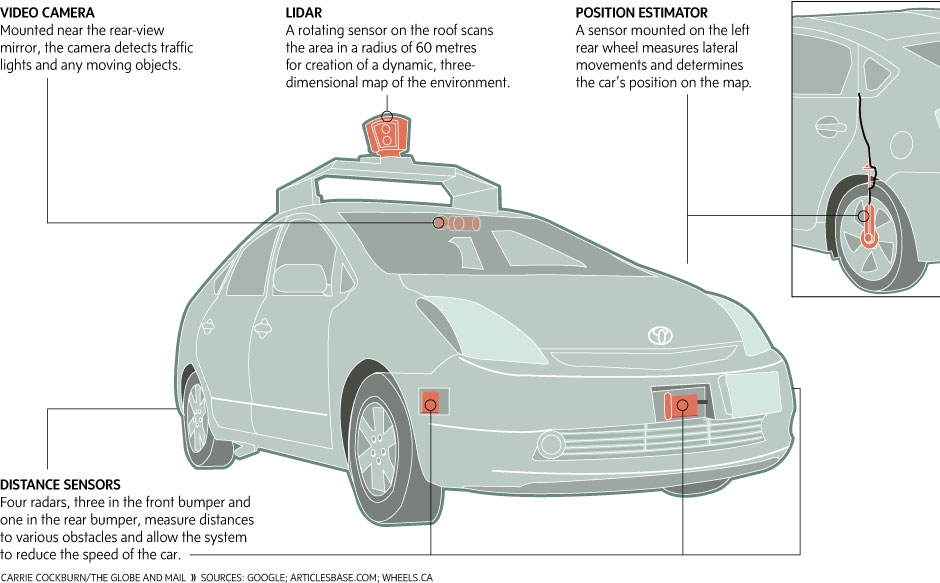
\includegraphics[width=\textwidth]{car-diagram}
\vspace{5mm}

Second, the car includes a powerful computer to analyze all these parameters
and actually \lq drive\rq the car. Let's take the example of Google's software
called \lq Chauffeur \rq . It's composed of two parts. One is hardcoded
(road signs, traffic lights colors), and one is a learning part. Every mile is
logged and provides additionnal data on how the car should drive itself.
Therefor, the car is able to predict the behavior of surrounding elements
(both car, bikes, pedestrians). Such things are based on neural networks behing
fed with the driving data of million of other cars
that Google has been collecting. This video by Google provides a great example
of how the car perceives its environment and can make decisions.

\vspace{5mm}
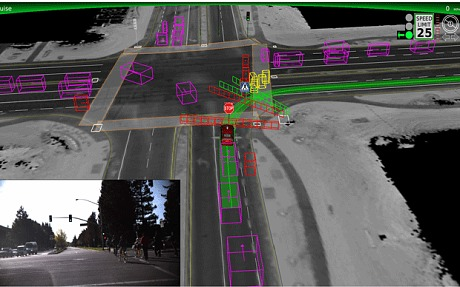
\includegraphics[width=\textwidth]{google-car}
How the Google car perceives its environment. More in video here: \url{https://www.youtube.com/watch?v=dk3oc1Hr62g}
\vspace{5mm}

\paragraph{Car industry discruption}
\\
The disruption is happening at several levels: some startups are building addons
to current cars, so they can get self-driving functionnalities. For instance,
a Californiancompany called Cruise
\footnote{\href{http://www.getcruise.com}{Cruise Website}}
enhances a car's capabilities by seamlessly integrating self-driving car
capabilities to your existing car. It works by adding sensors and a computer to
the car, and works in a similar fashion as the Google car. The idea is that you
can add those features to your car for about \$ 15,000 depending on the vehicle
you have. Google has a similar approach: according to several journalistic
sources, they intend to resell their self-driving technologies to automotive
companies. Though, many people fear that Google will have a significant
bargaining advantage, as those car companies don't have the technology yet.

Some other companies intend to replace current car makers. Tesla is the best
example in the category. Though the company CEO, Elon Musk, is confident
self-driving cars will hit the market by 2020, there were no public statement
about Tesla building such cars. In a recent video, he was asked whether Tesla
would be willing to provide Uber with self-driving cars, and declined to answer.
Many reporters concluded that Tesla will likely be the first company to sell
autonomous cars, that were built in-house. Similar to Tesla, there could be new
car giants rising by leverging the opportunity to build both a new type of car
and a powerful self-driving technology.

Finally, the most ambitious model is probably the one by Uber. The idea behind
it is that using UberX costs about \$ 2.15 per mile (source: AKA research).
Owning a personal car is \$ 0.76. Uber wants to create Car-As-a-Service.
The idea is similar to what Uber is today, but without the drivers. Think about
it for a moment. The car driver accounts for most of the cost of an UberX ride.
Therefore, if you can remove the driver, the cost would be \$ 0.25 per mile.
It's not only about replacing the driver, it's about making the car available
for customers at any time, on any day. Whereas a driver takes some rest and
parks their car, a self-driving car could be on the road almost 24/7.

\vspace{5mm}

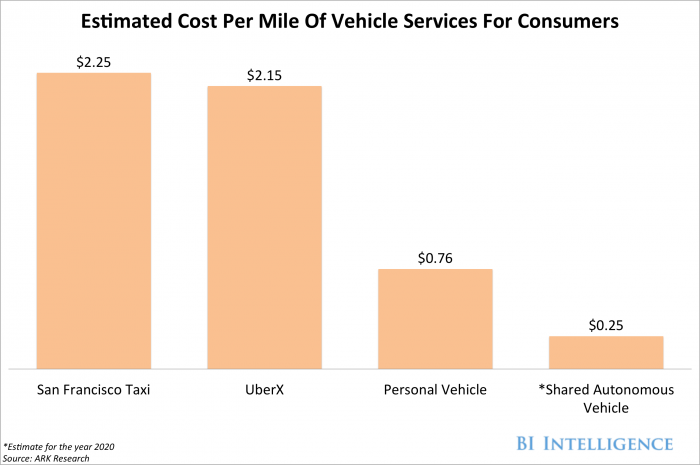
\includegraphics[width=\textwidth]{vehicle-cost}

\vspace{5mm}
No matter who's leading that change, it's likely that our own definition of the
car is going to change. Mercedes has shown an example of a car being similar to
a living room: the Mercedes-Benz F 015. Travellers could sleep, chat, browse the
internet as if they were at home. The car has been driving around San Francisco
this year.

\vspace{5mm}

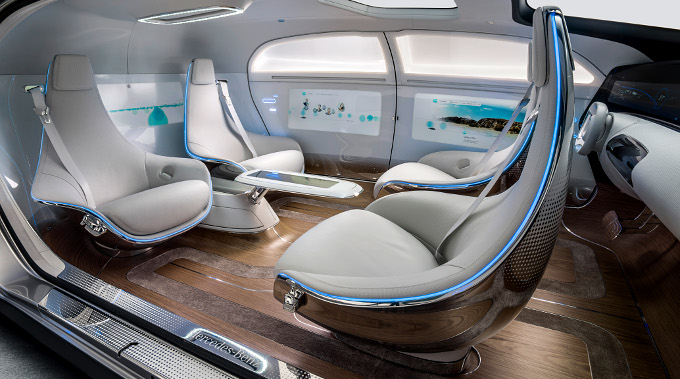
\includegraphics[width=\textwidth]{mercedes}

\vspace{5mm}

Another big change would be the oil station network. Since the car could drive
themselves to refill, or could be fully electricity powered, it will most likely
be the end of oil stations as we know them. Those will be probably automated as
well, and moved to non-residential areas.


\subsubsection{Speech \& natural-language recognition, or the death of interfaces}

The speech recognition movement has been initiated to the large public with a
startup bought by Apple, Siri. This startup was initiated a DARPA project as
well named CALO. Essentially, it works by transcripting speech to text, and then
parses the text to perform actions. Google has launched a similar service called
Google now. Both these system can perform actions based on the user's speech.
This technology enables the user to perform actions on the service of his
choosing (OpenTable, Yelp), without having to use any interface. The speech is
the communication tool.
\\
\paragraph{Technology behind it}
\\
Personal assistant technologies rely on three parts.
The first one is about extracting the meaning of the speech to figure out which
action to perform. In that case, Siri uses for instance part of speech tagging,
noun-phrase chunking, dependency \& constituent parsing. On the other side,
such service should plug into third party services. The complexity lies in the
ability to connect with very various systems (AirBnb, HotelTonight, Couchsurfing
,Bookking.com only to make a hotel reservation). Once this has been done, Siri
needs to communicate back with the user, converting API responses to oral \&
human communication.
\\
\paragraph{Use cases}
\\
Plenty of services have followed the Siri path, usually in a more advanced
fashion. It's interesting to note that some services are built with technology
at its core (Siri \& Google Now), whereas others are human-based at first. The Y
Combinator startup called \lq Magic\rq  is the exact opposite. The service only
includes the written language recognition. For instance, a user can text Magic
asking for anything they'd like, and then the service will connect to thirt
party services (in a similar fashion than Siri) to provide the service live. The
complexity therefore lies on relying on a very large number of 3rd party
services to provide a very large offering to the user. When a regular supermarket
has a limited inventory, Magic, as a personal assistant, needs to be able to
deliver anything the user wants. The second part of the complexity is scaling.
When you have human handling each operation at the beginning, you need to
progressively create processes to better handle certain tasks, and eventually
automate entire parts of the workflow.

Combining AI and diversity of requests doesn't seem to be possible today. Such
startups are having trouble to scale. The current solution is to combine a mix
of the two. Facebook Messenger recently launched a service called M that
illustrates it: they've leveraged the purchase of the French startup Wit.ai and
a team of personal assistants that handle manually some request to provide this
personal assistant service.

This market is likely a winner takes all one. Since these personal assistant
platforms are about connecting people with services, their model is similar to
Google's search engine. If you are the entry point for the customer, it's very
hard for competitors to make the users switch. Startups like Magic benefited
from their speed of execution, but the ability to scale requires to leverage AI
technology. It's not clear today whether startups or giants will succeed in that
field. Though it's interesting to see that the 2 take 2 opposite approach to
later converge in the same area.

Additional services from startup in that space intend to focus on one vertical
only. A good example of it are personal assistant focused on organizing meetings
between to person who want to schedule an appointment. To name a few, players in
that space are x.ai, assistant.ai or juliedesk. These companies are managing to
live up to their promise, but the complexity once again lies in the ability to
scale. They are strongly investing in AI to replace human services that they
first relied on.

Finally, we could imagine two models for that space.
One would be a model built by a major tech company (among Facebook, Google or
Apple) that would provide any kind of service by levering a strong AI
technology, and would plug into a very large number of APIs from company that
provide food delivery, order delivery, or pretty much anything.
The second model would be a platform one. A company like Magic could be the
entry point for the user. Then, if a calendar request is made to Magic, it would
just have to tag it as so and to route it to a Calendar booking service such as
x.ai.

The former seems more likely as concentrating the efforts in Machine Learning is
probably the best approach to achieve the best results, though the two are
possible.

\subsubsection{Death of interfaces}

The main benefit of such services for the user is that it's a very easy way to
communicate with a machine, in order to get a service. Think about the
User-Experience behind it. If you use a speech recognition, you would just
have to say: \lq Book me a table for 2 in a historic area of Paris, where I
can eat italian
food.\rq. That will do the trick.
If the user was to do it on their laptop or on their phone, they'll need to:
\begin{itemize}
  \item Find the right service to search on (TripAdivisor, OpenTable, Yelp?).
  \item Perform the search.
  \item Make a choice
  \item Go through the reservation process.
\end{itemize}

The former is way faster. Another benefit is in what we would call \lq unique\rq
cases. Say you want to book a laser-tag party in Paris, and you've never done it
before. You don't know where to look, so you're going to spend time figuring out
how to book a good laser-tag game. You'll probably need to benchmark a few,
look at the review, etc.

A strong case in favor of speech-based application is that you don't need to
learn about the existence of the service, and you don't need to use any
interface. UX designers often struggle to make an app available to all. No
interface is probably the most efficient. Even a 80 year-old who has never used
an app in their life would be able to use it. We can then imagine that, instead
of having dozens of apps on our phone or dozens of websites pinned on our
browsers, a single personal assistant app could do the job. Just like Google
does for search today. This user experience part make those personal assistant
particularly appealing in the long-run, because the friction to start using them
is very low. A good example of it we saw is about forwarding professional
expenses to the company's accountant. The mainstream service for it today is
Expensify. You just need to install an app on your phone (meaning, if you have
1000 people in the company, they all need to install it), then you can take a
picture of a receipt and it will automatically be sent to the company's
accoutant. This all process would be easier with a speech or written language
recognition app. You could just send over the receipt's picture via text to the
company AI bot. It will recognize what it is, potentially ask a few question
about the expense and done.

Time will tell, but usually the service that provides the simplest user
experience wins. And it's likely that the personal assistant user experience is
the simplest.


\subsubsection{The next generation of SaaS}

A new generation of SaaS is on the rise. The current SaaS solutions are comparable to toolboxes. They offer the ability to perform any action on any object. For instance, in the Salesforce interface (a CRM in SaaS for Sales people), you can basically customize the interface as much as you want so you can display any piece of information about a prospect.


\\
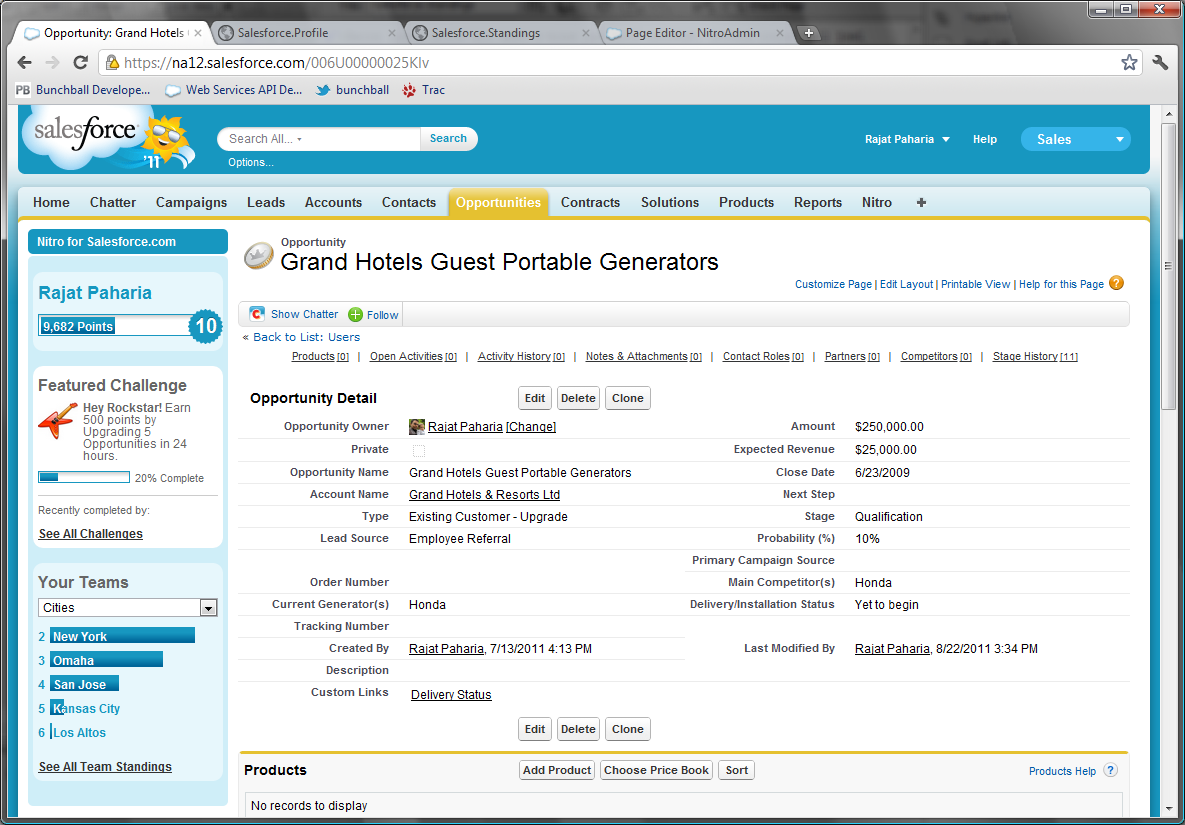
\includegraphics[width=\textwidth]{salesforce}
\\

The main challenge with those interfaces is that they end up being very crowded. There a second issue. The more information there is, the more complex it becomes to identify that you should perform an action. Say one of the metrics you use to track the customers usage of your application goes down. You may have a hundred metrics and miss this. Therefore, you won't be able to notice it.
SaaS CRM are great to manage a very large number of customers, but that comes with a price. The ability to pay a lot of attention to a given customer doesn't scale that easily.
There are some solutions. CRM like Salesforce, Zoho CRM, Zendesk and others provide the ability to create rules to identify specific behavior, so the user can be notified about certain events. Say a customer is about to churn because metric X is low, the sales rep will get a notification and will email the prospect.
All this sounds like it could be a good candidate for machine learning right? It is. A new generation of SaaS software is on the rise. This generation uses machine learning to automate those patterns. Essentially it can do two things: 1. is improving the user experience, and 2. is helping the user in regards to what to do to reach their goal.

\\
\paragraph{Smart interfaces}
\\

First, the user experience. We've seen that the interace of the current SaaS is usually crowded. That negatively impacts the productivity of the user, because they need to find the right piece of information they need among a ton of pieces of information. How could that be easier. Let's take the example of Zendesk, which is a CRM for customer support. Essentially, Zendesk is designed to respond to customers' inquiry, and to make it easy to satisfy those customers. The thing is, there are a ton of information, both available inside Zendesk, or in 3rd party services (e.g. the payment platform the company uses). Therefore, the customer support person needs to look around for the right piece of information, which takes time. Machine learning can help here. Companies like Gorgias.io, or Wise.io already display specific contextual buttons for the user to take actions according to the content of the message.

\\
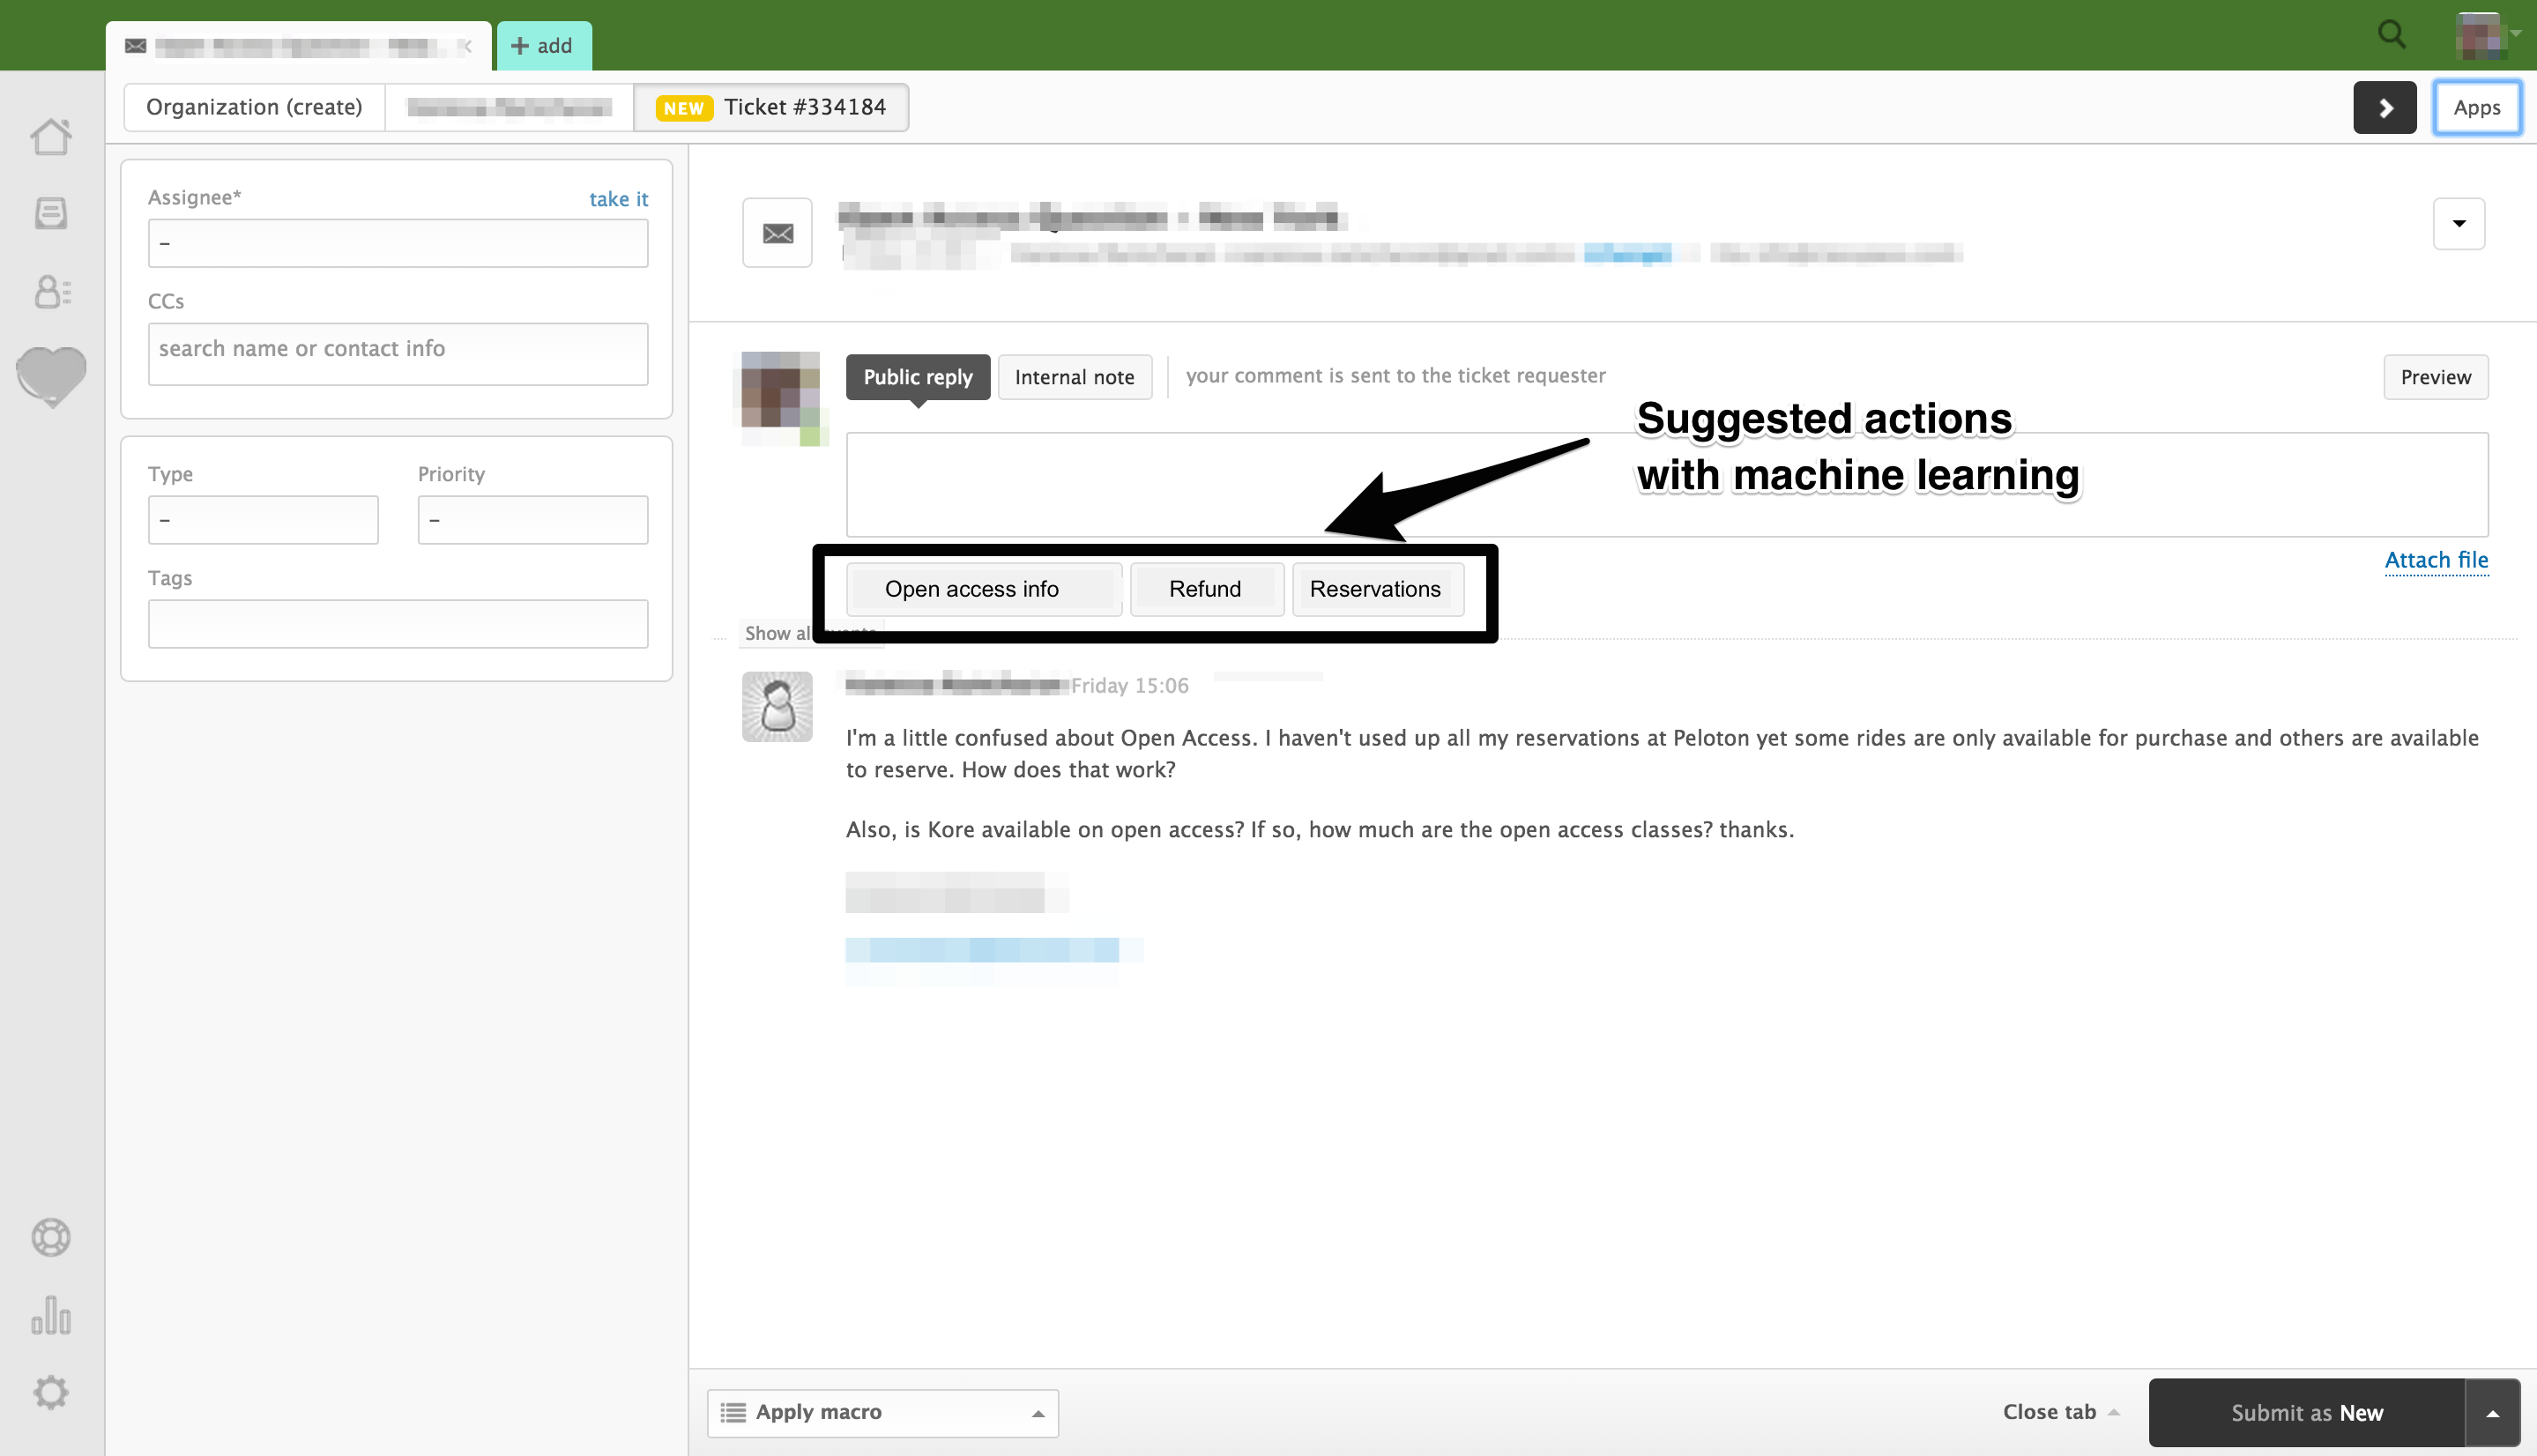
\includegraphics[width=\textwidth]{zendesk}
Gorgias can suggest the right canned response to a message
\\

It means when responding to a message, the support person doesn't have to look around for the right canned response. They are just suggested it by those smart pieces of software.
It could be the same with the information displayed in the interface. A customer request contains a large amount of information, that can help identify what piece of information will be needed by the customer support person to satisfy the request. On top of this, customer support is usually receiving hundreds of requests per day. Therefore, their could be tools that only show the right piece of information to the user, based on what is needed to resolve the case. One step further would be to suggest the right piece of information to the customer.

\\
\paragraph{Suggestions of actions}
\\

Second, we can expect the next generation of software for Enterprise businesses to be able to suggest actions and identify patterns by itself.\footnote{http://techcrunch.com/2015/07/27/the-next-wave-of-enterprise-software-powered-by-machine-learning} These services will be based on the collection of very large amount of data about a given customer. Then, it will be able to identify actions to be made in regards to the customer. A good example of it is identifying that a customer is ready to buy. A few SaaS services already provide that kind of intelligence: \href{http://www.gainsight.com/}{Gainsight} and \href{http://uk.insidesales.com/}{Insidesales} are good examples of it.
The main challenge they have is that they work as plugings. Therefore, their service is great, but cannot imapct the user experience of the sales person inside Salesforce for instance.
We can expect the next move in that sphere to be for Salesforce to integrate those capabilities. There are actually two ways to integrate them. The first is to add even more information in the interface to suggest or show those smart pieces of information / those suggestion of actions. The second is to integrate them in the user flow. Let say a user needs to send an invoice to a customer on a monthly. Salesforce could identify this, and figure out that customers who receive also stats usage while getting the invoice are less likely to churn. In that case, the software could suggest to not only send the invoice, but aslo send monthly usage statistics along with it, in the click of a button.
It's likely that unifying the user flow, which means the current course of actions the user takes in Salesforce, and the suggestions from machine learning algorithm would be the best way for users to adopt and use it. Therefor, the value will be captured by the companies which manage to unify machine learning suggestion in the current user flow.

\subsection{Impact on startup structures}

\subsubsection{The path to the full-software company}

If you look at how a SaaS business works today, you'll realize that the company essentially relies on a very large number of other SaaS services. For instance, it will use a SaaS platform for analytics (MixPanel, Kissmetrics, another for marketing (Marketo, Customer.io), another for CRM (Intercom, Salesforce) another to handle payments & accounting (Stripe, Octobat, Baremetrics), etc.
All this demonstrate one reality, each business unit in the company has its own SaaS platform, and they are all inter-connected. The step one was to provide each of those business units with a tool that facilitates their life. Step 2 is to automate those business units. A good example of it is Stripe, Baremetrics & Octobat. Those three SaaS combined can almost take care of all the payments, invoicing and sales reporting, without requiring a heavy setup not human intervention once they work. Octobat automatically invoices the customers according to the payments which were made or which are scheduled in Stripe. Baremetrics does the reporting out of the box.
\\

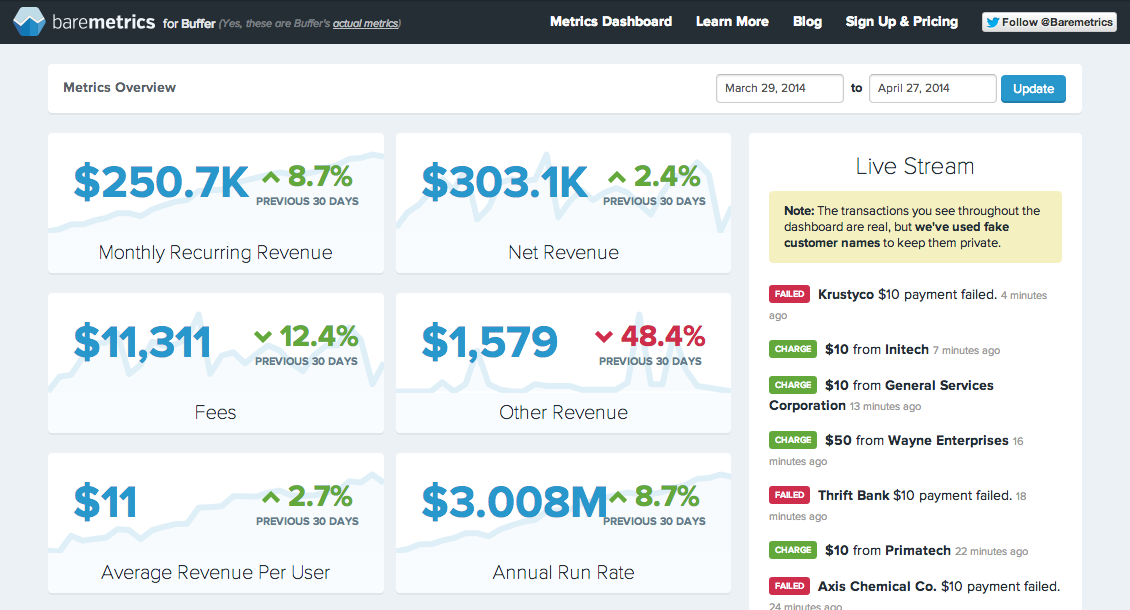
\includegraphics[width=\textwidth]{baremetrics}
Baremetrics provides business analytics out of the box for the company manager to monitor progress.
\\

One can guess that this behavior will expend to other areas of the business, that will be fully automated. Some people think it will only apply to blue collar work. But that's not the case. Project management can also be automated. Tools like \url{https://www.mturk.com/mturk/welcome}{Mechanical Turk} by Amazon enable to distribute work to remote contractors, and to achieve big projects at scale. Researchers have worked on a experiment: a basic AI software had to conduct a project from Scratch with this platform, by splitting the general task into small pieces that it hired contractors to do. This is probably also a glance at the future of a company: middle management will be automated.
\\

\paragraph{The Uber example}
\\

Probably the best example of this is Uber. A blog post by Peter Reinhardt\footnote{\href{http://rein.pk/replacing-middle-management-with-apis/}{Replacing Middle Management with APIs}} demonstrates that a big trend among tech businesses is to automate workloads distributions. Uber does it by providing end users to directly order a cab. If you think about the experience from the taxi driver experience, their workload is totally automated. They are assigned rides by Uber's algorithm, which they just need to execute. Same goes with other kinds of contractor work, for instance \url{https://www.getbannerman.com/}{Bannerman} provides the ability to book security gards on demand, without the middle man.
\vspace{5mm}
\\
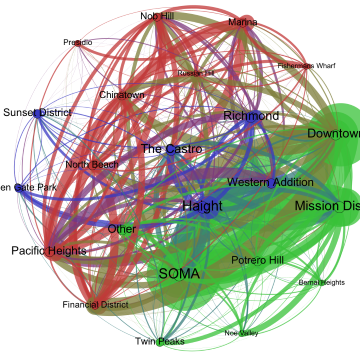
\includegraphics[width=\textwidth]{uber-graph}
Uber can predict taxi traffic based on historical data, and suggest drivers to go to the right place. This graph\url{http://blogs.mathworks.com/loren/2014/09/06/analyzing-uber-ride-sharing-gps-data/}{graph} shows the rides made by Uber drivers on weekends in San Francisco.
The size of the nodes represent the number of rides per location, hence their popularity.
The colors (green, blue, red) show which cluster a node belong to. Hence, you can predict in which area a taxi driver will drive: we'll most likely stay in the same cluster, and distribute the work accordingly.
\\

\paragraph{How to achieve a full-software company}
\\

There are two challenges related to building a full software company.
One is the ability to build a software for each business unit. We've seen that the startup ecosystem is making progress in that direction: Uber is doing it for the taxi workload management, Octobat for invoicing software. We can expect to see more and more pieces of software handling part of the business.
The second aspect of it is the ability to gather and share data. For a piece of software to do the full job of a business unit (say: accounting), the software needs to have access to all the data related to the business. Usually, this data is manually shared between services. To automate the process of sharing information, there's a need for a software that fully handles it.
We're good progress here. A company like \url{https://segment.com/}{Segment.com} handles it for analytics and user activity data. The admin just needs to install Segment on their website and define user events. Then, it will share this user data among a large amount of third party services through API integrations built by them. The user just need to activate a service on Segment for the data to be shared. It's that easy.
\\

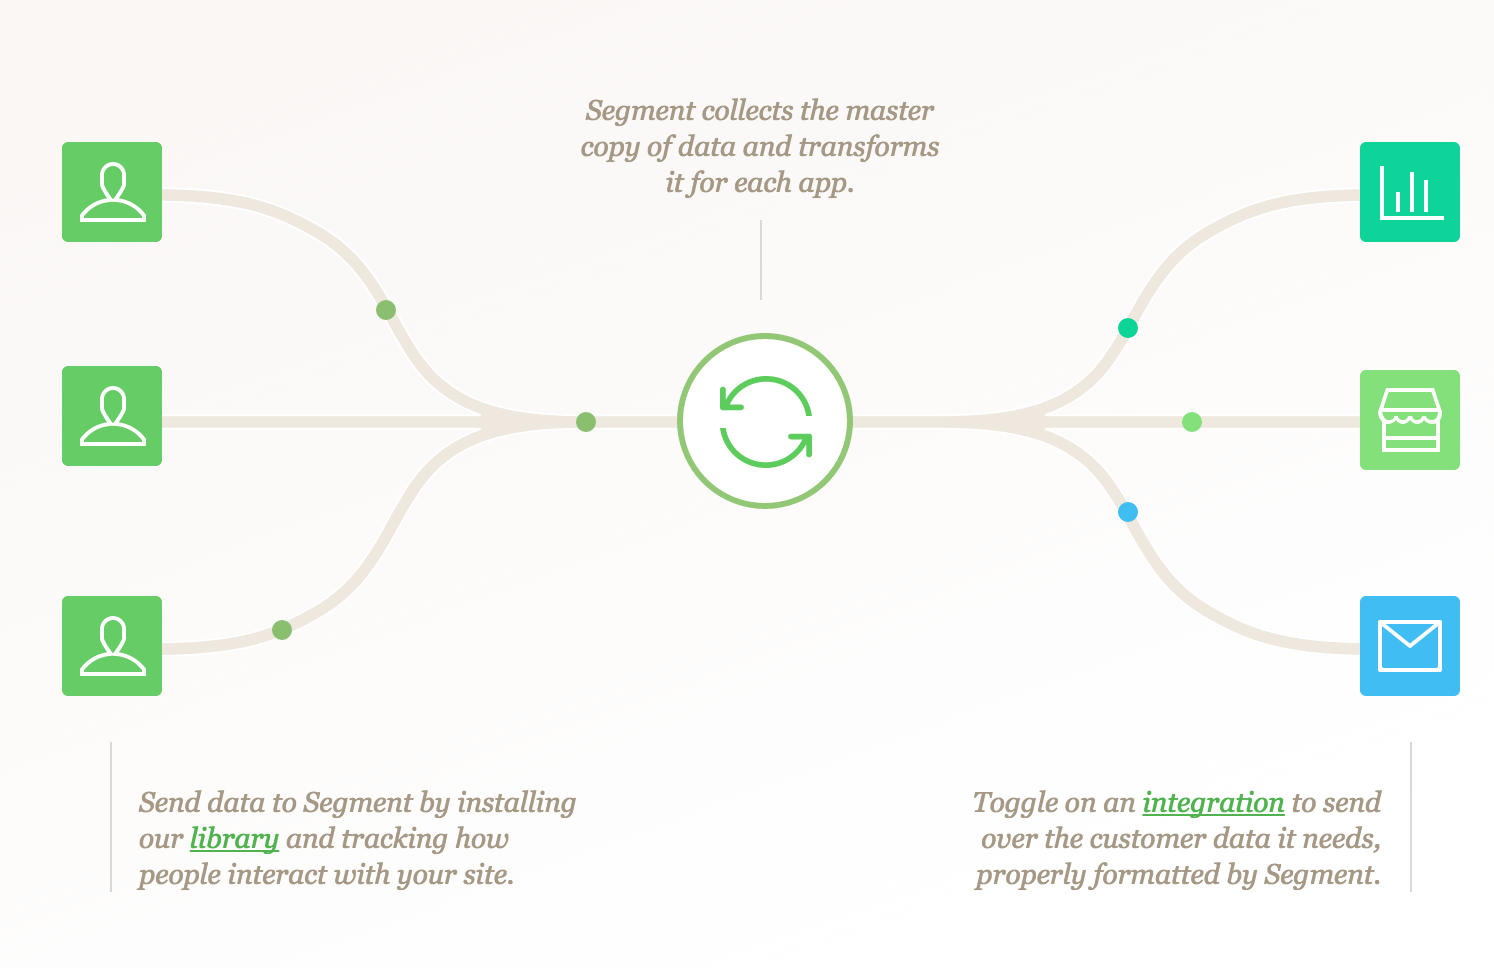
\includegraphics[width=\textwidth]{segment}
Services like Segment share data among all software a company has.
\\

We can expect to see similar services at the scope of the whole company. Think about the ability for a software not only tohave access to any piece of information about users or about the business, but also to be able to perform actions in third parties. Today, we're at the information sharing step, but soon we'll reach the latter.
Once it's possible to both share information and perform actions (e.g. offer them a refund after they experience a bug or raise a complaint), we'll reach one step further in the fully automated software company.
The human work may then focus on the creativity aspect of it, while it will be possible to fully autoamte the operational side of things.

\subsubsection{New kinds of business models}



\pagebreak
%%%%%%%%%%%%%%%%%%%%%%%%%%%%%%%%%%%%%%%%%%%%%%%%%%%%%%%%%%%%%%%%%%%%%%%%%%%%%%%%
%%%%%%%%%%%%%%%%%%%%%%%%%%%%%%% 3rd Part %%%%%%%%%%%%%%%%%%%%%%%%%%%%%%%%%%%%%%%
%%%%%%%%%%%%%%%%%%%%%%%%%%%%%%%%%%%%%%%%%%%%%%%%%%%%%%%%%%%%%%%%%%%%%%%%%%%%%%%%


\section{Limits}




Sources

\section{Car}

\url{http://www.google.com/selfdrivingcar/}
\url{http://www.businessinsider.com/why-uber-is-investing-in-autonomous-cars-2015-8?IR=T}
\url{http://www.entrepreneur.com/article/243751}
\url{http://www.forbes.com/sites/chunkamui/2014/08/04/5-reasons-why-automakers-should-fear-googles-driverless-car/}
\url{http://my.teslamotors.com/fr_CH/forum/forums/tesla%E2%80%99s-musk-sees-fully-autonomous-car-ready-5-years}

\section{Speech recognition}


\pagebreak

%%%%%%%%%%%%%%%%%%%%%%%%%%%%%%%%%%%%%%%%%%%%%%%%%%%%%%%%%%%%%%%%%%%%%%%%%%%%%%%%
%%%%%%%%%%%%%%%%%%%%%%%%%%%%%%% Conclusion %%%%%%%%%%%%%%%%%%%%%%%%%%%%%%%%%%%%%
%%%%%%%%%%%%%%%%%%%%%%%%%%%%%%%%%%%%%%%%%%%%%%%%%%%%%%%%%%%%%%%%%%%%%%%%%%%%%%%%

\section*{Conclusion}\label{conclusion}
\addcontentsline{toc}{section}{Conclusion}

\pagebreak


%%%%%%%%%%%%%%%%%%%%%%%%%%%%%%%%%%%%%%%%%%%%%%%%%%%%%%%%%%%%%%%%%%%%%%%%%%%%%%%%
%%%%%%%%%%%%%%%%%%%%%%%%%%%%%%% Bibliography %%%%%%%%%%%%%%%%%%%%%%%%%%%%%%%%%%%
%%%%%%%%%%%%%%%%%%%%%%%%%%%%%%%%%%%%%%%%%%%%%%%%%%%%%%%%%%%%%%%%%%%%%%%%%%%%%%%%

\begin{thebibliography}{40}

  \bibitem{seq2seq} Oriol Vinyal \& Quoc V. Le,
  {\em A Neural Conversation Model}, Google - June 2015

  \bibitem{Kurzweil} Ray Kurzweil, {\em The Singularity is near} - 2005

  \bibitem{Turing} Alan Turing, {\em The Imitation Game} - 1950

  \bibitem{Atari} DeepMind Technologies, {\em Playing Atari with Deep
  Reinforcement Learning} - 2015
  \bibitem{Good} Irving J. Good, {\em Advances in Computers, Vol 6} - 1965

  \bibitem{ChineseRoom} John Searle, {\em Minds, Brains, and Programs},
  Behavioral and Brain Sciences - 1980

  \bibitem{RusselAI} Stuart Russel \& Peter Norvig

  {\em Artificial Intelligence - A Modern Approach, 3rd Edition} - 2010.



\end{thebibliography}


\end{document}
